\documentclass[
  man,
  floatsintext,
  longtable,
  nolmodern,
  notxfonts,
  notimes,
  mask,
  colorlinks=true,linkcolor=blue,citecolor=blue,urlcolor=blue]{apa7}

\usepackage{amsmath}
\usepackage{amssymb}
\usepackage{setspace}



\RequirePackage{longtable}
\RequirePackage{threeparttablex}

\usepackage{framed}


\makeatletter
\renewcommand{\paragraph}{\@startsection{paragraph}{4}{\parindent}%
	{0\baselineskip \@plus 0.2ex \@minus 0.2ex}%
	{-.5em}%
	{\normalfont\normalsize\bfseries\typesectitle}}

\renewcommand{\subparagraph}[1]{\@startsection{subparagraph}{5}{0.5em}%
	{0\baselineskip \@plus 0.2ex \@minus 0.2ex}%
	{-\z@\relax}%
	{\normalfont\normalsize\bfseries\itshape\hspace{\parindent}{#1}\textit{\addperi}}{\relax}}
\makeatother




% longtable is already loaded via doc-class.tex (apa7 class option) and
% apatemplate.tex (\RequirePackage{longtable}). Keep booktabs here so raw
% LaTeX tables using \toprule/\midrule still render even without Pandoc table
% nodes.
\usepackage{booktabs, multirow, multicol, colortbl, hhline, caption, array, float, xpatch}
\usepackage{subcaption}


\renewcommand\thesubfigure{\Alph{subfigure}}
\setcounter{topnumber}{2}
\setcounter{bottomnumber}{2}
\setcounter{totalnumber}{4}
\renewcommand{\topfraction}{0.85}
\renewcommand{\bottomfraction}{0.85}
\renewcommand{\textfraction}{0.15}
\renewcommand{\floatpagefraction}{0.7}

\usepackage{tcolorbox}
\tcbuselibrary{listings,theorems, breakable, skins}
\usepackage{fontawesome5}

\definecolor{quarto-callout-color}{HTML}{909090}
\definecolor{quarto-callout-note-color}{HTML}{0758E5}
\definecolor{quarto-callout-important-color}{HTML}{CC1914}
\definecolor{quarto-callout-warning-color}{HTML}{EB9113}
\definecolor{quarto-callout-tip-color}{HTML}{00A047}
\definecolor{quarto-callout-caution-color}{HTML}{FC5300}
\definecolor{quarto-callout-color-frame}{HTML}{ACACAC}
\definecolor{quarto-callout-note-color-frame}{HTML}{4582EC}
\definecolor{quarto-callout-important-color-frame}{HTML}{D9534F}
\definecolor{quarto-callout-warning-color-frame}{HTML}{F0AD4E}
\definecolor{quarto-callout-tip-color-frame}{HTML}{02B875}
\definecolor{quarto-callout-caution-color-frame}{HTML}{FD7E14}

%\newlength\Oldarrayrulewidth
%\newlength\Oldtabcolsep


\usepackage{hyperref}
\usepackage[protrusion=true]{microtype}


\providecommand{\tightlist}{%
  \setlength{\itemsep}{0pt}\setlength{\parskip}{0pt}}
\usepackage{longtable,booktabs,array}
\usepackage{calc} % for calculating minipage widths
% Correct order of tables after \paragraph or \subparagraph
\usepackage{etoolbox}
\makeatletter
\patchcmd\longtable{\par}{\if@noskipsec\mbox{}\fi\par}{}{}
\makeatother
% Allow footnotes in longtable head/foot
\IfFileExists{footnotehyper.sty}{\usepackage{footnotehyper}}{\usepackage{footnote}}
\makesavenoteenv{longtable}

\usepackage{graphicx}
\makeatletter
\newsavebox\pandoc@box
\newcommand*\pandocbounded[1]{% scales image to fit in text height/width
  \sbox\pandoc@box{#1}%
  \Gscale@div\@tempa{\textheight}{\dimexpr\ht\pandoc@box+\dp\pandoc@box\relax}%
  \Gscale@div\@tempb{\linewidth}{\wd\pandoc@box}%
  \ifdim\@tempb\p@<\@tempa\p@\let\@tempa\@tempb\fi% select the smaller of both
  \ifdim\@tempa\p@<\p@\scalebox{\@tempa}{\usebox\pandoc@box}%
  \else\usebox{\pandoc@box}%
  \fi%
}
% Set default figure placement to htbp
\def\fps@figure{htbp}
\makeatother







\usepackage{newtx}

\defaultfontfeatures{Scale=MatchLowercase}
\defaultfontfeatures[\rmfamily]{Ligatures=TeX,Scale=1}





\title{Supplemental Material: Prompt Language Doesn't Matter, but Keep
the Original Text: Large Language Models and Sentiment Analysis in
French News}


\shorttitle{Supplemental Material}


\usepackage{etoolbox}






\author{Anonymized for review}



\affiliation{
{Anonymized for review}}




\leftheader{review}



\abstract{Supplemental tables and figures for the article. }

\keywords{supplemental material}

\authornote{ 

\par{       }
\par{Correspondence concerning this article should be addressed to }
}

\makeatletter
\let\endoldlt\endlongtable
\def\endlongtable{
\hline
\endoldlt
}
\makeatother

\urlstyle{same}



\usepackage{pdflscape}
\renewcommand{\thetable}{S\arabic{table}}
\renewcommand{\thefigure}{S\arabic{figure}}
\makeatletter
\@ifpackageloaded{caption}{}{\usepackage{caption}}
\AtBeginDocument{%
\ifdefined\contentsname
  \renewcommand*\contentsname{Table of contents}
\else
  \newcommand\contentsname{Table of contents}
\fi
\ifdefined\listfigurename
  \renewcommand*\listfigurename{List of Figures}
\else
  \newcommand\listfigurename{List of Figures}
\fi
\ifdefined\listtablename
  \renewcommand*\listtablename{List of Tables}
\else
  \newcommand\listtablename{List of Tables}
\fi
\ifdefined\figurename
  \renewcommand*\figurename{Figure}
\else
  \newcommand\figurename{Figure}
\fi
\ifdefined\tablename
  \renewcommand*\tablename{Table}
\else
  \newcommand\tablename{Table}
\fi
}
\@ifpackageloaded{float}{}{\usepackage{float}}
\floatstyle{ruled}
\@ifundefined{c@chapter}{\newfloat{codelisting}{h}{lop}}{\newfloat{codelisting}{h}{lop}[chapter]}
\floatname{codelisting}{Listing}
\newcommand*\listoflistings{\listof{codelisting}{List of Listings}}
\makeatother
\makeatletter
\makeatother
\makeatletter
\@ifpackageloaded{caption}{}{\usepackage{caption}}
\@ifpackageloaded{subcaption}{}{\usepackage{subcaption}}
\makeatother

% From https://tex.stackexchange.com/a/645996/211326
%%% apa7 doesn't want to add appendix section titles in the toc
%%% let's make it do it
\makeatletter
\xpatchcmd{\appendix}
  {\par}
  {\addcontentsline{toc}{section}{\@currentlabelname}\par}
  {}{}
\makeatother

%% Disable longtable counter
%% https://tex.stackexchange.com/a/248395/211326

\usepackage{etoolbox}

\makeatletter
\patchcmd{\LT@caption}
  {\bgroup}
  {\bgroup\global\LTpatch@captiontrue}
  {}{}
\patchcmd{\longtable}
  {\par}
  {\par\global\LTpatch@captionfalse}
  {}{}
\apptocmd{\endlongtable}
  {\ifLTpatch@caption\else\addtocounter{table}{-1}\fi}
  {}{}
\newif\ifLTpatch@caption
\makeatother

\begin{document}

\maketitle




\setlength\LTleft{0pt}



\ifdefined\Shaded\renewenvironment{Shaded}{\begin{snugshade}\begin{singlespace}}{\end{singlespace}\end{snugshade}}\fi


\ifdefined\cslhangindent\else\newlength{\cslhangindent}\fi
\ifdefined\csllabelwidth\else\newlength{\csllabelwidth}\fi
\setlength{\cslhangindent}{0.5in}


\begin{table}

{\caption{{Search Terms Used to Select Articles in the Eureka
Database}{\label{tbl-query}}}
\vspace{-20pt}}

\begin{longtable}[]{@{}
  >{\raggedright\arraybackslash}p{(\linewidth - 2\tabcolsep) * \real{0.1818}}
  >{\raggedright\arraybackslash}p{(\linewidth - 2\tabcolsep) * \real{0.8182}}@{}}
\toprule\noalign{}
\begin{minipage}[b]{\linewidth}\raggedright
Group
\end{minipage} & \begin{minipage}[b]{\linewidth}\raggedright
Search terms
\end{minipage} \\
\midrule\noalign{}
\endhead
\bottomrule\noalign{}
\endlastfoot
French terms & \emph{logiciel libre}, \emph{logiciels libres},
\emph{logiciel open source}, \emph{logiciels open source}, \emph{code
source ouvert}, \emph{code source libre} \\
English and borrowed terms & \emph{open source}, \emph{open-source},
\emph{free software}, \emph{software libre} \\
Proper names & \emph{Free Software Foundation}, \emph{Richard
Stallman} \\
\end{longtable}

\end{table}

\begin{table}

{\caption{{Collected Articles by Source
Media}{\label{tbl-source-summary}}}
\vspace{-20pt}}

\begin{longtable}[]{@{}llll@{}}
\toprule\noalign{}
Source & Articles & First article & Last article \\
\midrule\noalign{}
\endhead
\bottomrule\noalign{}
\endlastfoot
Libération & 769 & 1995-06-23 & 2024-11-04 \\
Monde, Le & 666 & 2001-01-09 & 2024-12-26 \\
Figaro, Le & 402 & 1998-10-21 & 2024-12-04 \\
Devoir, Le & 318 & 1998-07-20 & 2024-10-26 \\
Soleil, Le (Québec, QC) & 179 & 1998-11-08 & 2023-11-18 \\
Presse, La & 152 & 1998-03-26 & 2017-10-14 \\
Journal de Montréal, Le & 65 & 2006-12-20 & 2023-04-24 \\
Journal de Québec, Le & 45 & 2007-03-24 & 2024-10-19 \\
Tribune, La (Sherbrooke, QC) & 43 & 2000-03-29 & 2022-12-03 \\
Droit, Le (Ottawa, ON) & 17 & 1998-11-10 & 2014-07-17 \\
Nouvelliste, Le (Trois-Rivières, QC) & 13 & 2000-01-13 & 2022-03-05 \\
Quotidien, Le (Saguenay, QC) & 10 & 2008-11-01 & 2019-04-10 \\
Voix de l'Est, La (Granby, QC) & 4 & 2010-09-17 & 2015-02-14 \\
\end{longtable}

\end{table}

\begin{table}

{\caption{{Wording of the English and French Prompts on French Text, by
Component. Both Were Preceded by the Same English System Prompt: ``You
are a helpful assistant that analyzes the sentiment of text. You provide
accurate and consistent sentiment ratings according to the specified
scale.'' The English Prompt on the English Translation Differs Only in
Referring to English Instead of French (Task and Instruction
1).}{\label{tbl-prompt}}}
\vspace{-20pt}}

\begin{longtable}[]{@{}
  >{\raggedright\arraybackslash}p{(\linewidth - 4\tabcolsep) * \real{0.1395}}
  >{\raggedright\arraybackslash}p{(\linewidth - 4\tabcolsep) * \real{0.4302}}
  >{\raggedright\arraybackslash}p{(\linewidth - 4\tabcolsep) * \real{0.4302}}@{}}
\toprule\noalign{}
\begin{minipage}[b]{\linewidth}\raggedright
Component
\end{minipage} & \begin{minipage}[b]{\linewidth}\raggedright
English prompt
\end{minipage} & \begin{minipage}[b]{\linewidth}\raggedright
French prompt
\end{minipage} \\
\midrule\noalign{}
\endhead
\bottomrule\noalign{}
\endlastfoot
Task & Please analyze the sentiment of the following French text and
provide a single numerical rating according to this scale: & Veuillez
analyser le sentiment du texte français suivant et fournir une
évaluation numérique unique selon cette échelle : \\
Scale, -1.0 & Strong negative sentiment - highly critical, hostile, or
pessimistic content & Sentiment négatif fort - contenu très critique,
hostile ou pessimiste \\
Scale, -0.5 & Moderate negative sentiment - somewhat negative,
disapproving, or concerned content & Sentiment négatif modéré - contenu
plutôt négatif, désapprobateur ou préoccupant \\
Scale, 0.0 & Neutral sentiment - factual, balanced, or neither positive
nor negative content & Sentiment neutre - contenu factuel, équilibré, ou
ni positif ni négatif \\
Scale, 0.5 & Moderate positive sentiment - somewhat positive, approving,
or optimistic content & Sentiment positif modéré - contenu plutôt
positif, approbateur ou optimiste \\
Scale, 1.0 & Strong positive sentiment - highly supportive,
enthusiastic, or optimistic content & Sentiment positif fort - contenu
très favorable, enthousiaste ou optimiste \\
Intermediate values & You may also use values between these points for
intermediate sentiment levels (e.g., -0.7, 0.3). & Vous pouvez également
utiliser des valeurs intermédiaires entre ces points pour des niveaux de
sentiment intermédiaires (par exemple, -0.7, 0.3). \\
Instruction 1 & First, carefully read and understand the text,
considering cultural and linguistic nuances in French. & D'abord, lisez
attentivement et comprenez le texte, en tenant compte des nuances
culturelles et linguistiques en français. \\
Instruction 2 & Analyze the emotional tone, word choice, and overall
message. & Analysez le ton émotionnel, le choix des mots et le message
global. \\
Instruction 3 & Respond ONLY with a single numerical value between -1.0
and 1.0 that best represents the sentiment. & Répondez UNIQUEMENT avec
une valeur numérique unique entre -1.0 et 1.0 qui représente le mieux le
sentiment. \\
Instruction 4 & Do not include ANY explanations, analysis, or additional
text in your response. & N'incluez AUCUNE explication, analyse ou texte
supplémentaire dans votre réponse. \\
Input & Here is the text to analyze: {[}sentence{]} & Voici le texte à
analyser : {[}sentence{]} \\
\end{longtable}

\end{table}

\begin{table}[p]
\caption{Correlation With Human Judgments (With 95\% Confidence Interval), Mean Absolute Error, and Number of Sentences Scored, by Model and Condition}
\begin{center}
\footnotesize
\setlength{\tabcolsep}{5pt}
\begin{tabular}{llcrlrr}
\hline
\textbf{Model} & \textbf{Weights} & \textbf{Condition} & \textbf{r} & \textbf{95\% CI} & \textbf{MAE} & \textbf{n} \\
\hline
GPT-5.6 Luna & Closed & FR→FR & 0.810 & [0.76, 0.85] & 0.168 & 200 \\
GPT-5.6 Luna & Closed & EN→FR & 0.802 & [0.75, 0.85] & 0.165 & 200 \\
GPT-5.6 Luna & Closed & EN→EN & 0.728 & [0.66, 0.79] & 0.176 & 200 \\
Jev 1.13 & Closed & FR→FR & 0.772 & [0.71, 0.82] & 0.163 & 200 \\
Jev 1.13 & Closed & EN→FR & 0.772 & [0.71, 0.82] & 0.169 & 200 \\
Jev 1.13 & Closed & EN→EN & 0.752 & [0.68, 0.81] & 0.176 & 200 \\
Gemini 3.5 Flash & Closed & FR→FR & 0.760 & [0.69, 0.81] & 0.170 & 200 \\
Gemini 3.5 Flash & Closed & EN→FR & 0.773 & [0.71, 0.82] & 0.162 & 200 \\
Gemini 3.5 Flash & Closed & EN→EN & 0.760 & [0.69, 0.81] & 0.165 & 200 \\
Claude Haiku 4.5 & Closed & FR→FR & 0.785 & [0.73, 0.83] & 0.182 & 200 \\
Claude Haiku 4.5 & Closed & EN→FR & 0.780 & [0.72, 0.83] & 0.185 & 200 \\
Claude Haiku 4.5 & Closed & EN→EN & 0.705 & [0.63, 0.77] & 0.182 & 200 \\
Qwen3 235B-A22B & Open & FR→FR & 0.774 & [0.71, 0.82] & 0.226 & 200 \\
Qwen3 235B-A22B & Open & EN→FR & 0.753 & [0.69, 0.81] & 0.232 & 200 \\
Qwen3 235B-A22B & Open & EN→EN & 0.680 & [0.60, 0.75] & 0.229 & 200 \\
GPT-OSS 120B & Open & FR→FR & 0.727 & [0.65, 0.79] & 0.205 & 200 \\
GPT-OSS 120B & Open & EN→FR & 0.743 & [0.67, 0.80] & 0.182 & 200 \\
GPT-OSS 120B & Open & EN→EN & 0.729 & [0.66, 0.79] & 0.172 & 200 \\
GPT-OSS 20B & Open & FR→FR & 0.733 & [0.66, 0.79] & 0.171 & 200 \\
GPT-OSS 20B & Open & EN→FR & 0.718 & [0.64, 0.78] & 0.191 & 200 \\
GPT-OSS 20B & Open & EN→EN & 0.695 & [0.62, 0.76] & 0.176 & 200 \\
Mistral Small 3.2 & Open & FR→FR & 0.735 & [0.66, 0.79] & 0.263 & 200 \\
Mistral Small 3.2 & Open & EN→FR & 0.728 & [0.66, 0.79] & 0.294 & 200 \\
Mistral Small 3.2 & Open & EN→EN & 0.669 & [0.58, 0.74] & 0.272 & 200 \\
DeepSeek V3.2 & Open & FR→FR & 0.686 & [0.61, 0.75] & 0.203 & 200 \\
DeepSeek V3.2 & Open & EN→FR & 0.743 & [0.67, 0.80] & 0.176 & 200 \\
DeepSeek V3.2 & Open & EN→EN & 0.683 & [0.60, 0.75] & 0.178 & 200 \\
Mistral Large 4 & Closed & FR→FR & 0.702 & [0.62, 0.77] & 0.184 & 200 \\
Mistral Large 4 & Closed & EN→FR & 0.713 & [0.64, 0.78] & 0.176 & 200 \\
Mistral Large 4 & Closed & EN→EN & 0.692 & [0.61, 0.76] & 0.169 & 200 \\
Qwen3 32B & Open & FR→FR & 0.679 & [0.60, 0.75] & 0.175 & 200 \\
Qwen3 32B & Open & EN→FR & 0.695 & [0.62, 0.76] & 0.170 & 200 \\
Qwen3 32B & Open & EN→EN & 0.644 & [0.56, 0.72] & 0.187 & 200 \\
Llama 4 Scout & Open & FR→FR & 0.644 & [0.55, 0.72] & 0.275 & 200 \\
Llama 4 Scout & Open & EN→FR & 0.661 & [0.58, 0.73] & 0.286 & 200 \\
Llama 4 Scout & Open & EN→EN & 0.618 & [0.52, 0.70] & 0.299 & 200 \\
Llama 3.1 8B & Open & FR→FR & 0.612 & [0.52, 0.69] & 0.273 & 199 \\
Llama 3.1 8B & Open & EN→FR & 0.604 & [0.51, 0.68] & 0.268 & 200 \\
Llama 3.1 8B & Open & EN→EN & 0.575 & [0.47, 0.66] & 0.254 & 200 \\
Lexicoder (EN) & Dictionary & EN & 0.548 & [0.44, 0.64] & 0.203 & 200 \\
Lexicoder (FR) & Dictionary & FR & 0.357 & [0.23, 0.47] & 0.210 & 200 \\
Llama 3.2 3B & Open & FR→FR & 0.476 & [0.36, 0.58] & 0.262 & 200 \\
Llama 3.2 3B & Open & EN→FR & 0.132 & [-0.01, 0.27] & 0.377 & 200 \\
Llama 3.2 3B & Open & EN→EN & 0.302 & [0.17, 0.42] & 0.305 & 200 \\
Llama 3.2 1B & Open & FR→FR & 0.100 & [-0.16, 0.35] & 0.551 & 58 \\
Llama 3.2 1B & Open & EN→FR & 0.003 & [-0.23, 0.23] & 0.604 & 74 \\
Llama 3.2 1B & Open & EN→EN & -0.199 & [-0.42, 0.05] & 0.526 & 66 \\
\hline
\end{tabular}

\end{center}
\end{table}
\clearpage

\begin{table}

{\caption{{Cost of Scoring 1,000 Sentences at List Prices (Upper Bound;
Cached Prompt Tokens Counted at the Full Input Rate; Input Tokens and
Cost Not Reported for Llama 3.2 1B, Whose Endpoint Returned a Constant
Token Count)}{\label{tbl-cost}}}
\vspace{-20pt}}

\begin{longtable}[]{@{}
  >{\raggedright\arraybackslash}p{(\linewidth - 12\tabcolsep) * \real{0.2405}}
  >{\raggedright\arraybackslash}p{(\linewidth - 12\tabcolsep) * \real{0.1392}}
  >{\raggedright\arraybackslash}p{(\linewidth - 12\tabcolsep) * \real{0.0886}}
  >{\raggedleft\arraybackslash}p{(\linewidth - 12\tabcolsep) * \real{0.1266}}
  >{\raggedleft\arraybackslash}p{(\linewidth - 12\tabcolsep) * \real{0.1266}}
  >{\raggedleft\arraybackslash}p{(\linewidth - 12\tabcolsep) * \real{0.1266}}
  >{\raggedleft\arraybackslash}p{(\linewidth - 12\tabcolsep) * \real{0.1519}}@{}}
\toprule\noalign{}
\begin{minipage}[b]{\linewidth}\raggedright
Model
\end{minipage} & \begin{minipage}[b]{\linewidth}\raggedright
Provider
\end{minipage} & \begin{minipage}[b]{\linewidth}\raggedright
Weights
\end{minipage} & \begin{minipage}[b]{\linewidth}\raggedleft
API calls per score
\end{minipage} & \begin{minipage}[b]{\linewidth}\raggedleft
Input tokens
\end{minipage} & \begin{minipage}[b]{\linewidth}\raggedleft
Output tokens
\end{minipage} & \begin{minipage}[b]{\linewidth}\raggedleft
USD per 1,000 sentences
\end{minipage} \\
\midrule\noalign{}
\endhead
\bottomrule\noalign{}
\endlastfoot
GPT-OSS 20B & OpenRouter & Open & 1.02 & 657,496 & 87,892 & 0.018 \\
Llama 3.2 3B & OpenRouter & Open & 1.00 & 595,142 & 7,320 & 0.018 \\
Jev 1.13 & TypeSafe & Closed & 1.00 & 815,199 & 32,400 & 0.019 \\
GPT-OSS 120B & OpenRouter & Open & 1.00 & 667,425 & 95,660 & 0.020 \\
Qwen3 32B & OpenRouter & Open & 1.00 & 592,086 & 5,696 & 0.027 \\
Mistral Small 3.2 & OpenRouter & Open & 1.00 & 553,761 & 7,405 &
0.029 \\
Qwen3 235B-A22B & OpenRouter & Open & 1.00 & 584,886 & 7,752 & 0.030 \\
Llama 4 Scout & OpenRouter & Open & 1.00 & 564,947 & 8,467 & 0.059 \\
DeepSeek V3.2 & OpenRouter & Open & 1.00 & 559,594 & 9,340 & 0.067 \\
Llama 3.1 8B & OpenRouter & Open & 1.01 & 593,398 & 8,062 & 0.074 \\
GPT-5.6 Luna & OpenAI & Closed & 1.00 & 552,225 & 51,819 & 0.096 \\
Mistral Large 4 & OpenRouter & Closed & 1.00 & 534,990 & 7,603 &
0.211 \\
Claude Haiku 4.5 & Anthropic & Closed & 1.00 & 648,705 & 12,600 &
0.395 \\
Gemini 3.5 Flash & Google & Closed & 1.04 & 572,330 & 577,590 & 3.365 \\
Llama 3.2 1B & OpenRouter & Open & 22.68 & -- & 168,789 & -- \\
\end{longtable}

\end{table}

\begin{table}

{\caption{{F1 Scores for 3-Category
Classification}{\label{tbl-f1-3cat}}}
\vspace{-20pt}}

\begin{longtable}[]{@{}lllll@{}}
\toprule\noalign{}
Model & Negative & Neutral & Positive & Weighted F1 \\
\midrule\noalign{}
\endhead
\bottomrule\noalign{}
\endlastfoot
Claude Haiku 4.5 (FR→FR) & 0.762 & 0.353 & 0.834 & 0.770 \\
GPT-5.6 Luna (FR→FR) & 0.748 & 0.400 & 0.811 & 0.756 \\
Jev 1.13 (EN→FR) & 0.691 & 0.444 & 0.821 & 0.748 \\
Jev 1.13 (FR→FR) & 0.695 & 0.357 & 0.814 & 0.738 \\
GPT-5.6 Luna (EN→FR) & 0.730 & 0.345 & 0.787 & 0.732 \\
Claude Haiku 4.5 (EN→FR) & 0.690 & 0.290 & 0.789 & 0.715 \\
Jev 1.13 (EN→EN) & 0.711 & 0.200 & 0.787 & 0.713 \\
Mistral Small 3.2 (FR→FR) & 0.578 & 0.250 & 0.832 & 0.703 \\
DeepSeek V3.2 (FR→FR) & 0.672 & 0.300 & 0.766 & 0.697 \\
Mistral Small 3.2 (EN→FR) & 0.545 & 0.320 & 0.829 & 0.697 \\
Qwen3 235B-A22B (FR→FR) & 0.752 & 0.260 & 0.727 & 0.695 \\
GPT-5.6 Luna (EN→EN) & 0.688 & 0.349 & 0.746 & 0.694 \\
DeepSeek V3.2 (EN→FR) & 0.696 & 0.250 & 0.748 & 0.689 \\
GPT-OSS 120B (FR→FR) & 0.721 & 0.301 & 0.722 & 0.686 \\
Llama 4 Scout (FR→FR) & 0.643 & 0.310 & 0.748 & 0.678 \\
Qwen3 235B-A22B (EN→FR) & 0.719 & 0.243 & 0.717 & 0.677 \\
Mistral Small 3.2 (EN→EN) & 0.488 & 0.320 & 0.824 & 0.675 \\
Llama 4 Scout (EN→FR) & 0.667 & 0.277 & 0.733 & 0.673 \\
GPT-OSS 120B (EN→FR) & 0.717 & 0.312 & 0.700 & 0.672 \\
Claude Haiku 4.5 (EN→EN) & 0.678 & 0.247 & 0.725 & 0.670 \\
GPT-OSS 20B (EN→FR) & 0.700 & 0.282 & 0.687 & 0.657 \\
GPT-OSS 20B (FR→FR) & 0.691 & 0.271 & 0.691 & 0.655 \\
Llama 4 Scout (EN→EN) & 0.647 & 0.233 & 0.696 & 0.641 \\
DeepSeek V3.2 (EN→EN) & 0.672 & 0.246 & 0.657 & 0.626 \\
Mistral Large 4 (EN→EN) & 0.604 & 0.242 & 0.687 & 0.623 \\
Gemini 3.5 Flash (EN→EN) & 0.667 & 0.244 & 0.653 & 0.622 \\
Llama 3.1 8B (EN→FR) & 0.652 & 0.269 & 0.656 & 0.622 \\
Mistral Large 4 (FR→FR) & 0.644 & 0.250 & 0.660 & 0.620 \\
Llama 3.1 8B (EN→EN) & 0.627 & 0.279 & 0.663 & 0.619 \\
Gemini 3.5 Flash (FR→FR) & 0.649 & 0.253 & 0.649 & 0.615 \\
Mistral Large 4 (EN→FR) & 0.648 & 0.229 & 0.642 & 0.609 \\
Gemini 3.5 Flash (EN→FR) & 0.661 & 0.231 & 0.630 & 0.606 \\
Llama 3.2 3B (FR→FR) & 0.465 & 0.182 & 0.733 & 0.602 \\
Llama 3.1 8B (FR→FR) & 0.615 & 0.163 & 0.653 & 0.602 \\
GPT-OSS 20B (EN→EN) & 0.614 & 0.227 & 0.646 & 0.600 \\
Qwen3 235B-A22B (EN→EN) & 0.698 & 0.220 & 0.601 & 0.599 \\
Lexicoder (EN) & 0.574 & 0.243 & 0.646 & 0.589 \\
GPT-OSS 120B (EN→EN) & 0.678 & 0.231 & 0.562 & 0.570 \\
Qwen3 32B (EN→FR) & 0.554 & 0.179 & 0.631 & 0.568 \\
Qwen3 32B (FR→FR) & 0.515 & 0.207 & 0.620 & 0.552 \\
Lexicoder (FR) & 0.474 & 0.279 & 0.620 & 0.545 \\
Qwen3 32B (EN→EN) & 0.559 & 0.202 & 0.529 & 0.511 \\
Llama 3.2 3B (EN→EN) & 0.167 & 0.245 & 0.717 & 0.503 \\
Llama 3.2 3B (EN→FR) & 0.000 & 0.200 & 0.745 & 0.464 \\
Llama 3.2 1B (FR→FR) & 0.000 & 0.194 & 0.638 & 0.423 \\
Llama 3.2 1B (EN→FR) & 0.000 & 0.057 & 0.558 & 0.321 \\
Llama 3.2 1B (EN→EN) & 0.000 & 0.146 & 0.435 & 0.268 \\
\end{longtable}

\end{table}

\clearpage
\begin{landscape}
\begin{table}[h]
\caption{F1 Scores for 7-Category Classification}
\begin{center}
\scriptsize
\setlength{\tabcolsep}{5pt}
\renewcommand{\arraystretch}{0.95}
\begin{tabular}{lcccccccc}
\hline
\textbf{Model} & \textbf{Very neg.} & \textbf{Negative} & \textbf{Somewhat neg.} & \textbf{Neutral} & \textbf{Somewhat pos.} & \textbf{Positive} & \textbf{Very pos.} & \textbf{Weighted F1} \\
\hline
Claude Haiku 4.5 (FR→FR) & 0.400 & 0.680 & 0.455 & 0.375 & 0.540 & 0.612 & 0.000 & 0.537 \\
Jev 1.13 (EN→FR) & 0.200 & 0.586 & 0.282 & 0.500 & 0.623 & 0.548 & 0.250 & 0.528 \\
Jev 1.13 (FR→FR) & 0.222 & 0.621 & 0.324 & 0.400 & 0.601 & 0.540 & 0.250 & 0.523 \\
Jev 1.13 (EN→EN) & 0.200 & 0.525 & 0.385 & 0.222 & 0.610 & 0.566 & 0.286 & 0.518 \\
GPT-5.6 Luna (FR→FR) & 0.286 & 0.500 & 0.393 & 0.385 & 0.538 & 0.462 & 0.133 & 0.479 \\
GPT-5.6 Luna (EN→EN) & 0.364 & 0.500 & 0.338 & 0.367 & 0.510 & 0.542 & 0.250 & 0.470 \\
GPT-5.6 Luna (EN→FR) & 0.333 & 0.500 & 0.258 & 0.364 & 0.564 & 0.407 & 0.125 & 0.455 \\
DeepSeek V3.2 (EN→EN) & 0.333 & 0.533 & 0.419 & 0.258 & 0.415 & 0.588 & 0.667 & 0.448 \\
Claude Haiku 4.5 (EN→EN) & 0.286 & 0.642 & 0.400 & 0.256 & 0.409 & 0.568 & 0.000 & 0.448 \\
GPT-OSS 120B (EN→FR) & 0.333 & 0.566 & 0.400 & 0.324 & 0.416 & 0.485 & 0.133 & 0.434 \\
Mistral Large 4 (EN→EN) & 0.333 & 0.651 & 0.316 & 0.250 & 0.444 & 0.408 & 0.000 & 0.423 \\
DeepSeek V3.2 (EN→FR) & 0.444 & 0.667 & 0.429 & 0.226 & 0.349 & 0.493 & 0.000 & 0.416 \\
Mistral Small 3.2 (EN→EN) & 0.333 & 0.345 & 0.222 & 0.364 & 0.549 & 0.364 & 0.091 & 0.416 \\
Mistral Large 4 (EN→FR) & 0.167 & 0.600 & 0.357 & 0.235 & 0.361 & 0.590 & 0.286 & 0.416 \\
DeepSeek V3.2 (FR→FR) & 0.333 & 0.368 & 0.469 & 0.216 & 0.400 & 0.527 & 0.167 & 0.415 \\
Claude Haiku 4.5 (EN→FR) & 0.500 & 0.680 & 0.364 & 0.273 & 0.347 & 0.511 & 0.200 & 0.413 \\
Mistral Large 4 (FR→FR) & 0.154 & 0.488 & 0.344 & 0.259 & 0.397 & 0.561 & 0.222 & 0.412 \\
Mistral Small 3.2 (FR→FR) & 0.500 & 0.400 & 0.170 & 0.286 & 0.509 & 0.380 & 0.125 & 0.394 \\
GPT-OSS 20B (EN→FR) & 0.235 & 0.431 & 0.269 & 0.268 & 0.370 & 0.535 & 0.000 & 0.376 \\
GPT-OSS 120B (EN→EN) & 0.444 & 0.692 & 0.281 & 0.218 & 0.288 & 0.536 & 0.286 & 0.373 \\
Gemini 3.5 Flash (FR→FR) & 0.222 & 0.583 & 0.250 & 0.264 & 0.310 & 0.571 & 0.200 & 0.370 \\
GPT-OSS 120B (FR→FR) & 0.308 & 0.545 & 0.333 & 0.314 & 0.319 & 0.447 & 0.154 & 0.369 \\
GPT-OSS 20B (FR→FR) & 0.364 & 0.600 & 0.286 & 0.258 & 0.325 & 0.448 & 0.286 & 0.367 \\
GPT-OSS 20B (EN→EN) & 0.400 & 0.528 & 0.235 & 0.234 & 0.338 & 0.508 & 0.000 & 0.362 \\
Gemini 3.5 Flash (EN→FR) & 0.400 & 0.694 & 0.255 & 0.242 & 0.263 & 0.485 & 0.167 & 0.349 \\
Qwen3 32B (EN→FR) & 0.222 & 0.512 & 0.163 & 0.165 & 0.286 & 0.615 & 0.000 & 0.334 \\
Qwen3 235B-A22B (FR→FR) & 0.190 & 0.407 & 0.320 & 0.243 & 0.319 & 0.369 & 0.087 & 0.330 \\
Mistral Small 3.2 (EN→FR) & 0.364 & 0.312 & 0.133 & 0.364 & 0.420 & 0.292 & 0.062 & 0.326 \\
Gemini 3.5 Flash (EN→EN) & 0.364 & 0.652 & 0.222 & 0.233 & 0.230 & 0.500 & 0.000 & 0.324 \\
Qwen3 32B (FR→FR) & 0.333 & 0.558 & 0.125 & 0.177 & 0.236 & 0.632 & 0.000 & 0.315 \\
Qwen3 235B-A22B (EN→FR) & 0.182 & 0.321 & 0.240 & 0.254 & 0.350 & 0.339 & 0.091 & 0.315 \\
Qwen3 235B-A22B (EN→EN) & 0.182 & 0.275 & 0.302 & 0.227 & 0.279 & 0.408 & 0.133 & 0.299 \\
Llama 3.1 8B (EN→FR) & 0.111 & 0.120 & 0.192 & 0.281 & 0.319 & 0.507 & 0.200 & 0.297 \\
Lexicoder (FR) & 0.000 & 0.000 & 0.253 & 0.289 & 0.479 & 0.057 & 0.000 & 0.290 \\
Llama 4 Scout (FR→FR) & 0.125 & 0.167 & 0.182 & 0.291 & 0.341 & 0.356 & 0.100 & 0.286 \\
Lexicoder (EN) & 0.000 & 0.000 & 0.267 & 0.231 & 0.472 & 0.000 & 0.000 & 0.276 \\
Llama 3.1 8B (FR→FR) & 0.143 & 0.197 & 0.179 & 0.174 & 0.239 & 0.543 & 0.000 & 0.267 \\
Llama 3.2 3B (FR→FR) & 0.000 & 0.364 & 0.200 & 0.195 & 0.240 & 0.395 & 0.000 & 0.266 \\
Qwen3 32B (EN→EN) & 0.222 & 0.364 & 0.172 & 0.190 & 0.168 & 0.567 & 0.333 & 0.261 \\
Llama 3.1 8B (EN→EN) & 0.138 & 0.222 & 0.136 & 0.265 & 0.246 & 0.479 & 0.143 & 0.261 \\
Llama 4 Scout (EN→FR) & 0.154 & 0.261 & 0.143 & 0.258 & 0.281 & 0.329 & 0.080 & 0.257 \\
Llama 4 Scout (EN→EN) & 0.105 & 0.280 & 0.125 & 0.246 & 0.234 & 0.434 & 0.154 & 0.252 \\
Llama 3.2 3B (EN→EN) & 0.000 & 0.138 & 0.050 & 0.261 & 0.250 & 0.375 & 0.000 & 0.217 \\
Llama 3.2 3B (EN→FR) & 0.000 & 0.000 & 0.000 & 0.222 & 0.232 & 0.317 & 0.000 & 0.171 \\
Llama 3.2 1B (EN→EN) & 0.000 & 0.000 & 0.000 & 0.150 & 0.000 & 0.211 & 0.000 & 0.051 \\
Llama 3.2 1B (FR→FR) & 0.000 & 0.000 & 0.000 & 0.138 & 0.000 & 0.000 & 0.000 & 0.007 \\
Llama 3.2 1B (EN→FR) & 0.000 & 0.000 & 0.000 & 0.000 & 0.000 & 0.000 & 0.000 & 0.000 \\
\hline
\end{tabular}

\end{center}
\end{table}
\end{landscape}
\clearpage

\begin{table}

{\caption{{Mean Input Tokens per API Call by Language Condition, and
Tokens per Word by Text Language (Valid Calls Only; Llama 3.2 1B
Excluded Because Its Endpoint Reported a Constant Token Count on Every
Call; Jev's Input Is a Structured Question Rather Than the Text Prompt,
So Its Counts Are Not Comparable)}{\label{tbl-tokens}}}
\vspace{-20pt}}

\begin{longtable}[]{@{}
  >{\raggedright\arraybackslash}p{(\linewidth - 12\tabcolsep) * \real{0.2785}}
  >{\raggedleft\arraybackslash}p{(\linewidth - 12\tabcolsep) * \real{0.0886}}
  >{\raggedleft\arraybackslash}p{(\linewidth - 12\tabcolsep) * \real{0.0886}}
  >{\raggedleft\arraybackslash}p{(\linewidth - 12\tabcolsep) * \real{0.0886}}
  >{\raggedleft\arraybackslash}p{(\linewidth - 12\tabcolsep) * \real{0.2025}}
  >{\raggedleft\arraybackslash}p{(\linewidth - 12\tabcolsep) * \real{0.1266}}
  >{\raggedleft\arraybackslash}p{(\linewidth - 12\tabcolsep) * \real{0.1266}}@{}}
\toprule\noalign{}
\begin{minipage}[b]{\linewidth}\raggedright
Model
\end{minipage} & \begin{minipage}[b]{\linewidth}\raggedleft
EN→EN
\end{minipage} & \begin{minipage}[b]{\linewidth}\raggedleft
EN→FR
\end{minipage} & \begin{minipage}[b]{\linewidth}\raggedleft
FR→FR
\end{minipage} & \begin{minipage}[b]{\linewidth}\raggedleft
French-prompt overhead
\end{minipage} & \begin{minipage}[b]{\linewidth}\raggedleft
Tokens per French word
\end{minipage} & \begin{minipage}[b]{\linewidth}\raggedleft
Tokens per English word
\end{minipage} \\
\midrule\noalign{}
\endhead
\bottomrule\noalign{}
\endlastfoot
Mistral Large 4 & 284.5 & 289.1 & 318.1 & +29 (+10.0\%) & 1.38 & 1.22 \\
Jev 1.13 & 431.0 & 440.3 & 487.3 & +47 (+10.7\%) & 1.62 & 1.22 \\
GPT-OSS 120B & 352.0 & 357.7 & 402.7 & +45 (+12.6\%) & 1.42 & 1.19 \\
GPT-OSS 20B & 339.0 & 344.7 & 389.7 & +45 (+13.1\%) & 1.42 & 1.19 \\
Llama 4 Scout & 294.1 & 299.9 & 343.9 & +44 (+14.7\%) & 1.41 & 1.19 \\
Mistral Small 3.2 & 288.6 & 294.6 & 339.6 & +45 (+15.3\%) & 1.45 &
1.22 \\
GPT-5.6 Luna & 288.0 & 293.7 & 338.7 & +45 (+15.3\%) & 1.42 & 1.19 \\
Gemini 3.5 Flash & 285.0 & 292.1 & 337.1 & +45 (+15.4\%) & 1.46 &
1.17 \\
Qwen3 32B & 296.5 & 307.7 & 382.7 & +75 (+24.4\%) & 1.69 & 1.21 \\
DeepSeek V3.2 & 280.1 & 290.3 & 361.3 & +71 (+24.5\%) & 1.61 & 1.19 \\
Qwen3 235B-A22B & 292.5 & 303.7 & 378.7 & +75 (+24.7\%) & 1.69 & 1.21 \\
Llama 3.2 3B & 295.2 & 306.8 & 388.8 & +82 (+26.7\%) & 1.69 & 1.20 \\
Llama 3.1 8B & 295.2 & 306.8 & 389.0 & +82 (+26.8\%) & 1.69 & 1.20 \\
Claude Haiku 4.5 & 313.8 & 328.2 & 439.2 & +111 (+33.8\%) & 1.87 &
1.25 \\
\end{longtable}

\end{table}

\begin{figure}[!htbp]

{\caption{{Correlation and Mean Absolute Error Between Model Scores and
Human Judgments, by Model and Condition}{\label{fig-s-performance}}}}

\pandocbounded{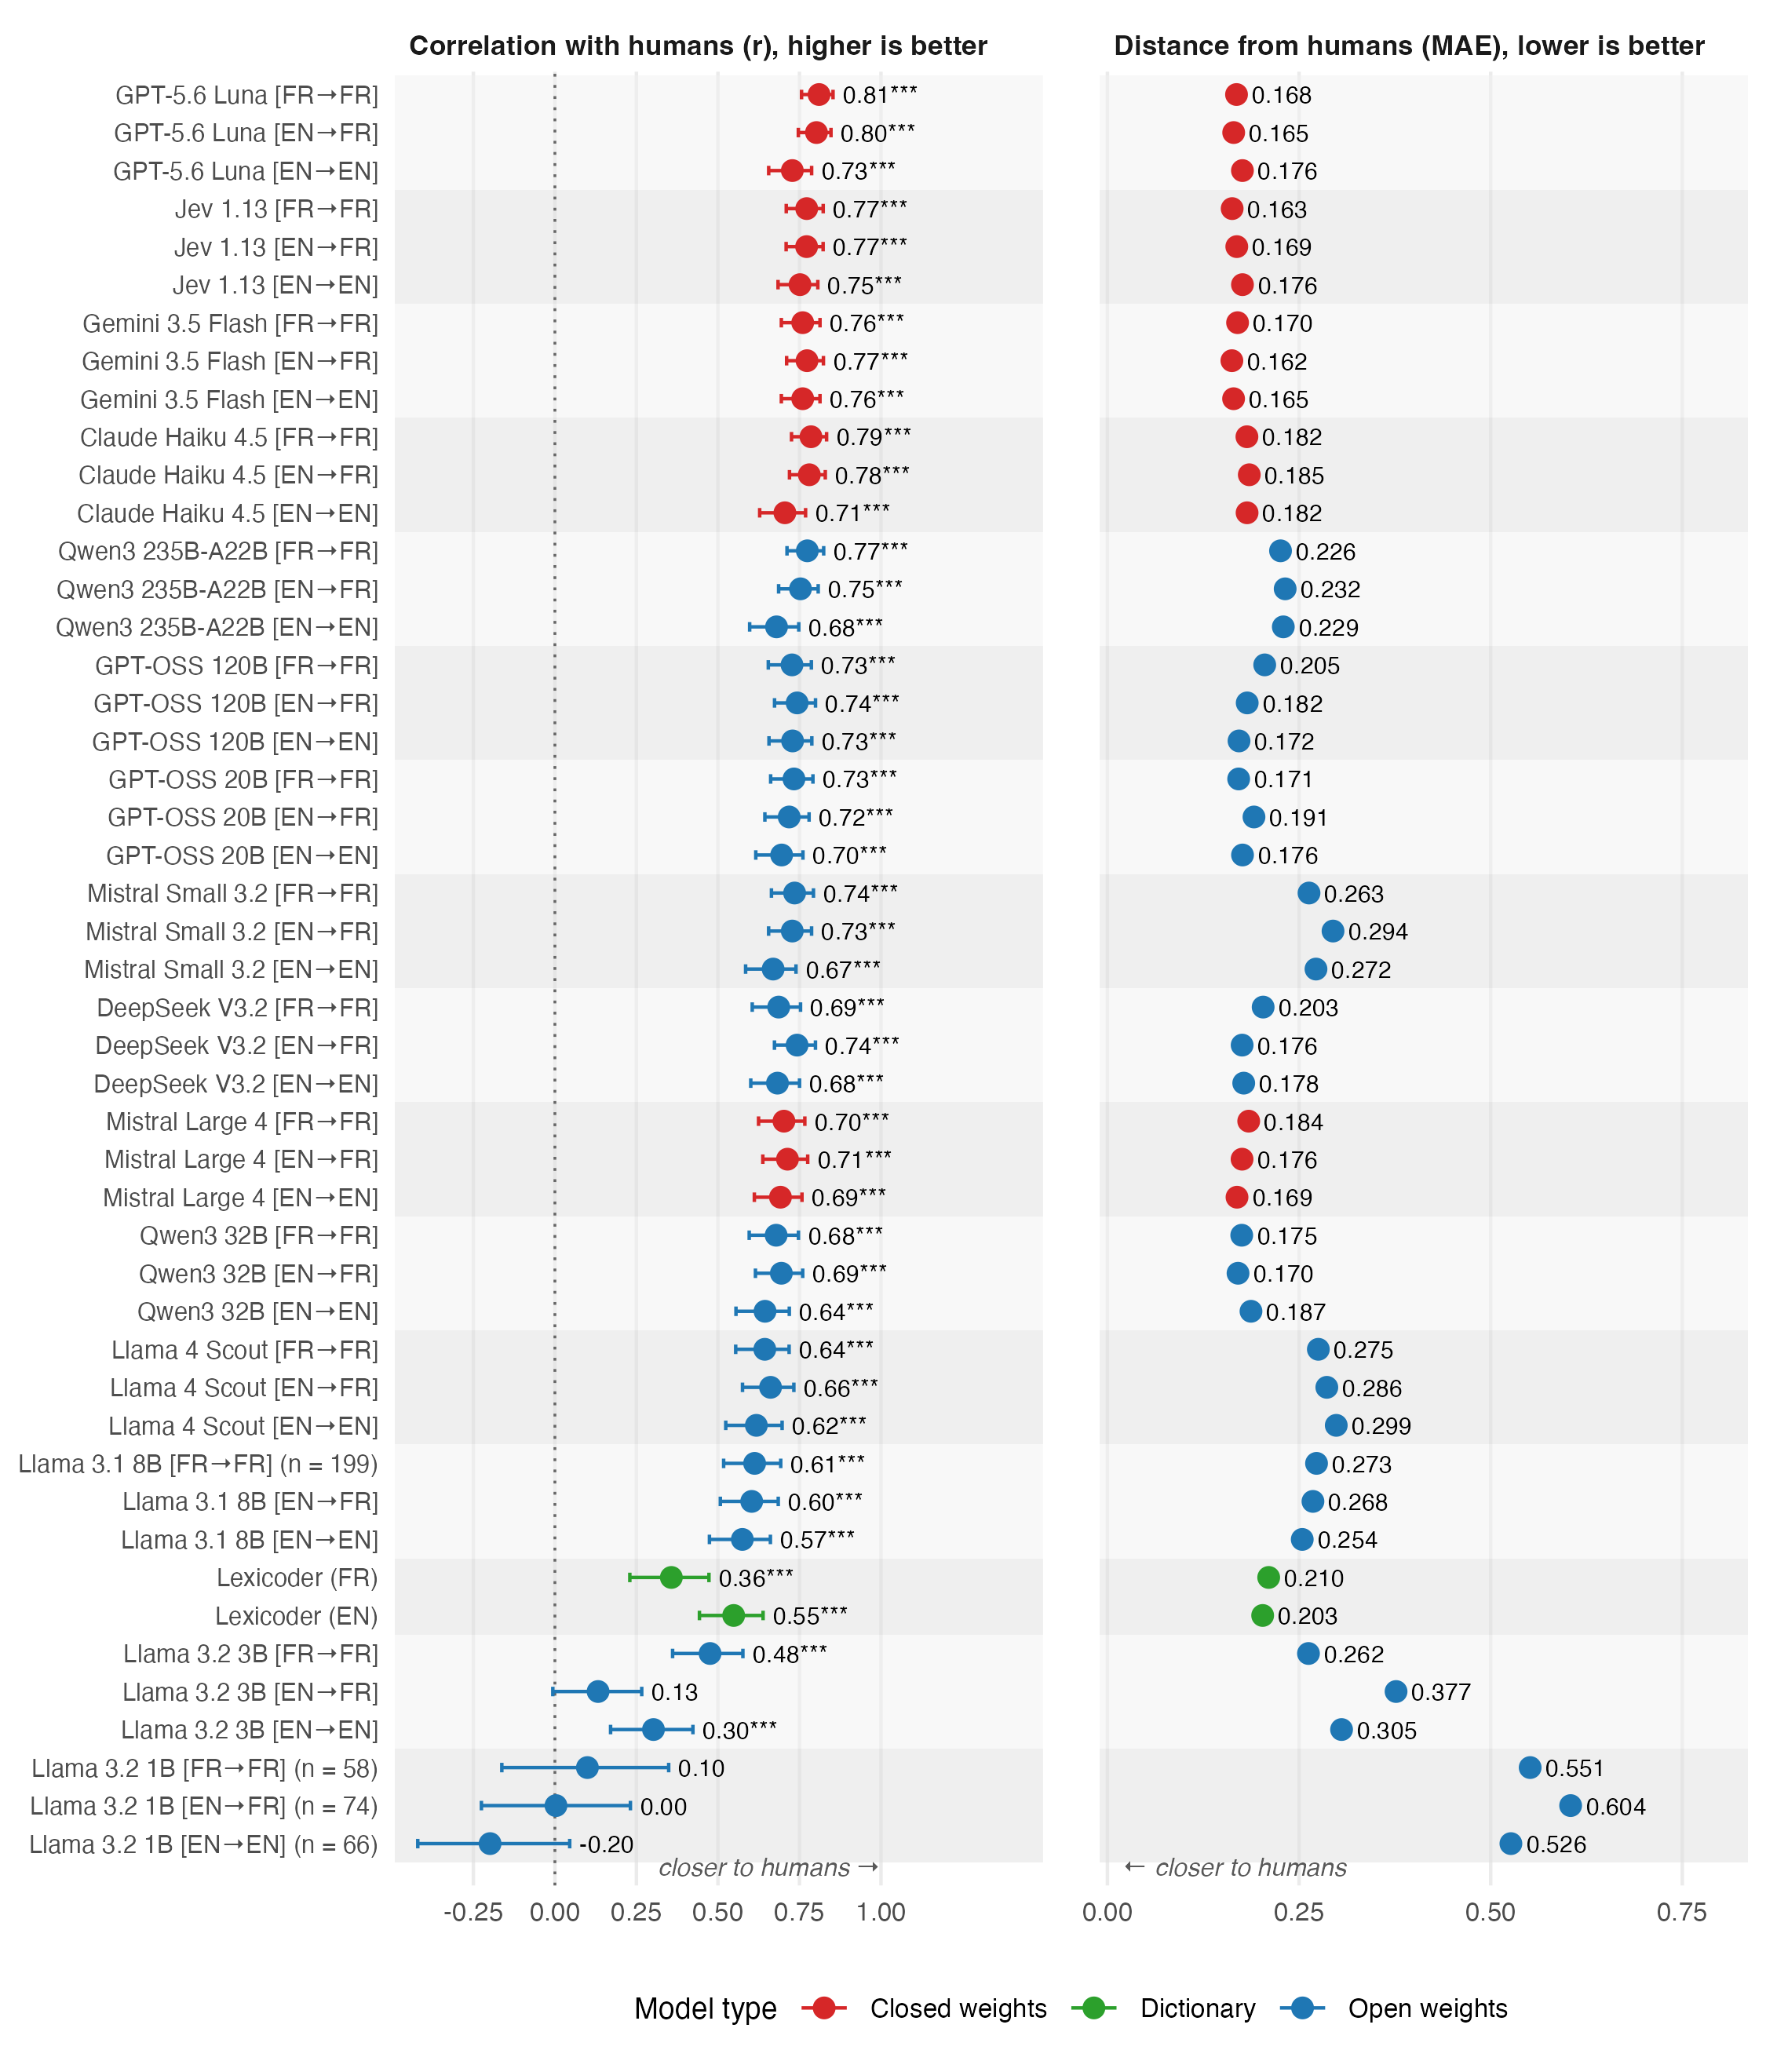
\includegraphics[keepaspectratio]{../../results/graphs/model_performance.png}}

\vspace{-12pt}
\noindent \emph{Note.} One~row per model and condition, sorted by each
model's mean correlation and colored by model type. Left panel: Pearson
correlation between the model's scores and the mean of three human
coders, with 95\% confidence intervals. Right panel: mean absolute
error, the average distance between the model's score and the human
score on the −1 to 1 scale, so that 0.17 means the model is typically
0.17 points away from the human rating. Within each model, the
conditions are FR→FR (French prompt on French text), EN→FR (English
prompt on French text), and EN→EN (English prompt on translated text).
\(^{*}p\) \textless{} .05, \(^{**}p\) \textless{} .01, \(^{***}p\)
\textless{} .001.

\end{figure}

\begin{figure}[!htbp]

{\caption{{Weighted F1 on Polarity and on Fine-Grained Classification,
by Model}{\label{fig-s-f1}}}}

\pandocbounded{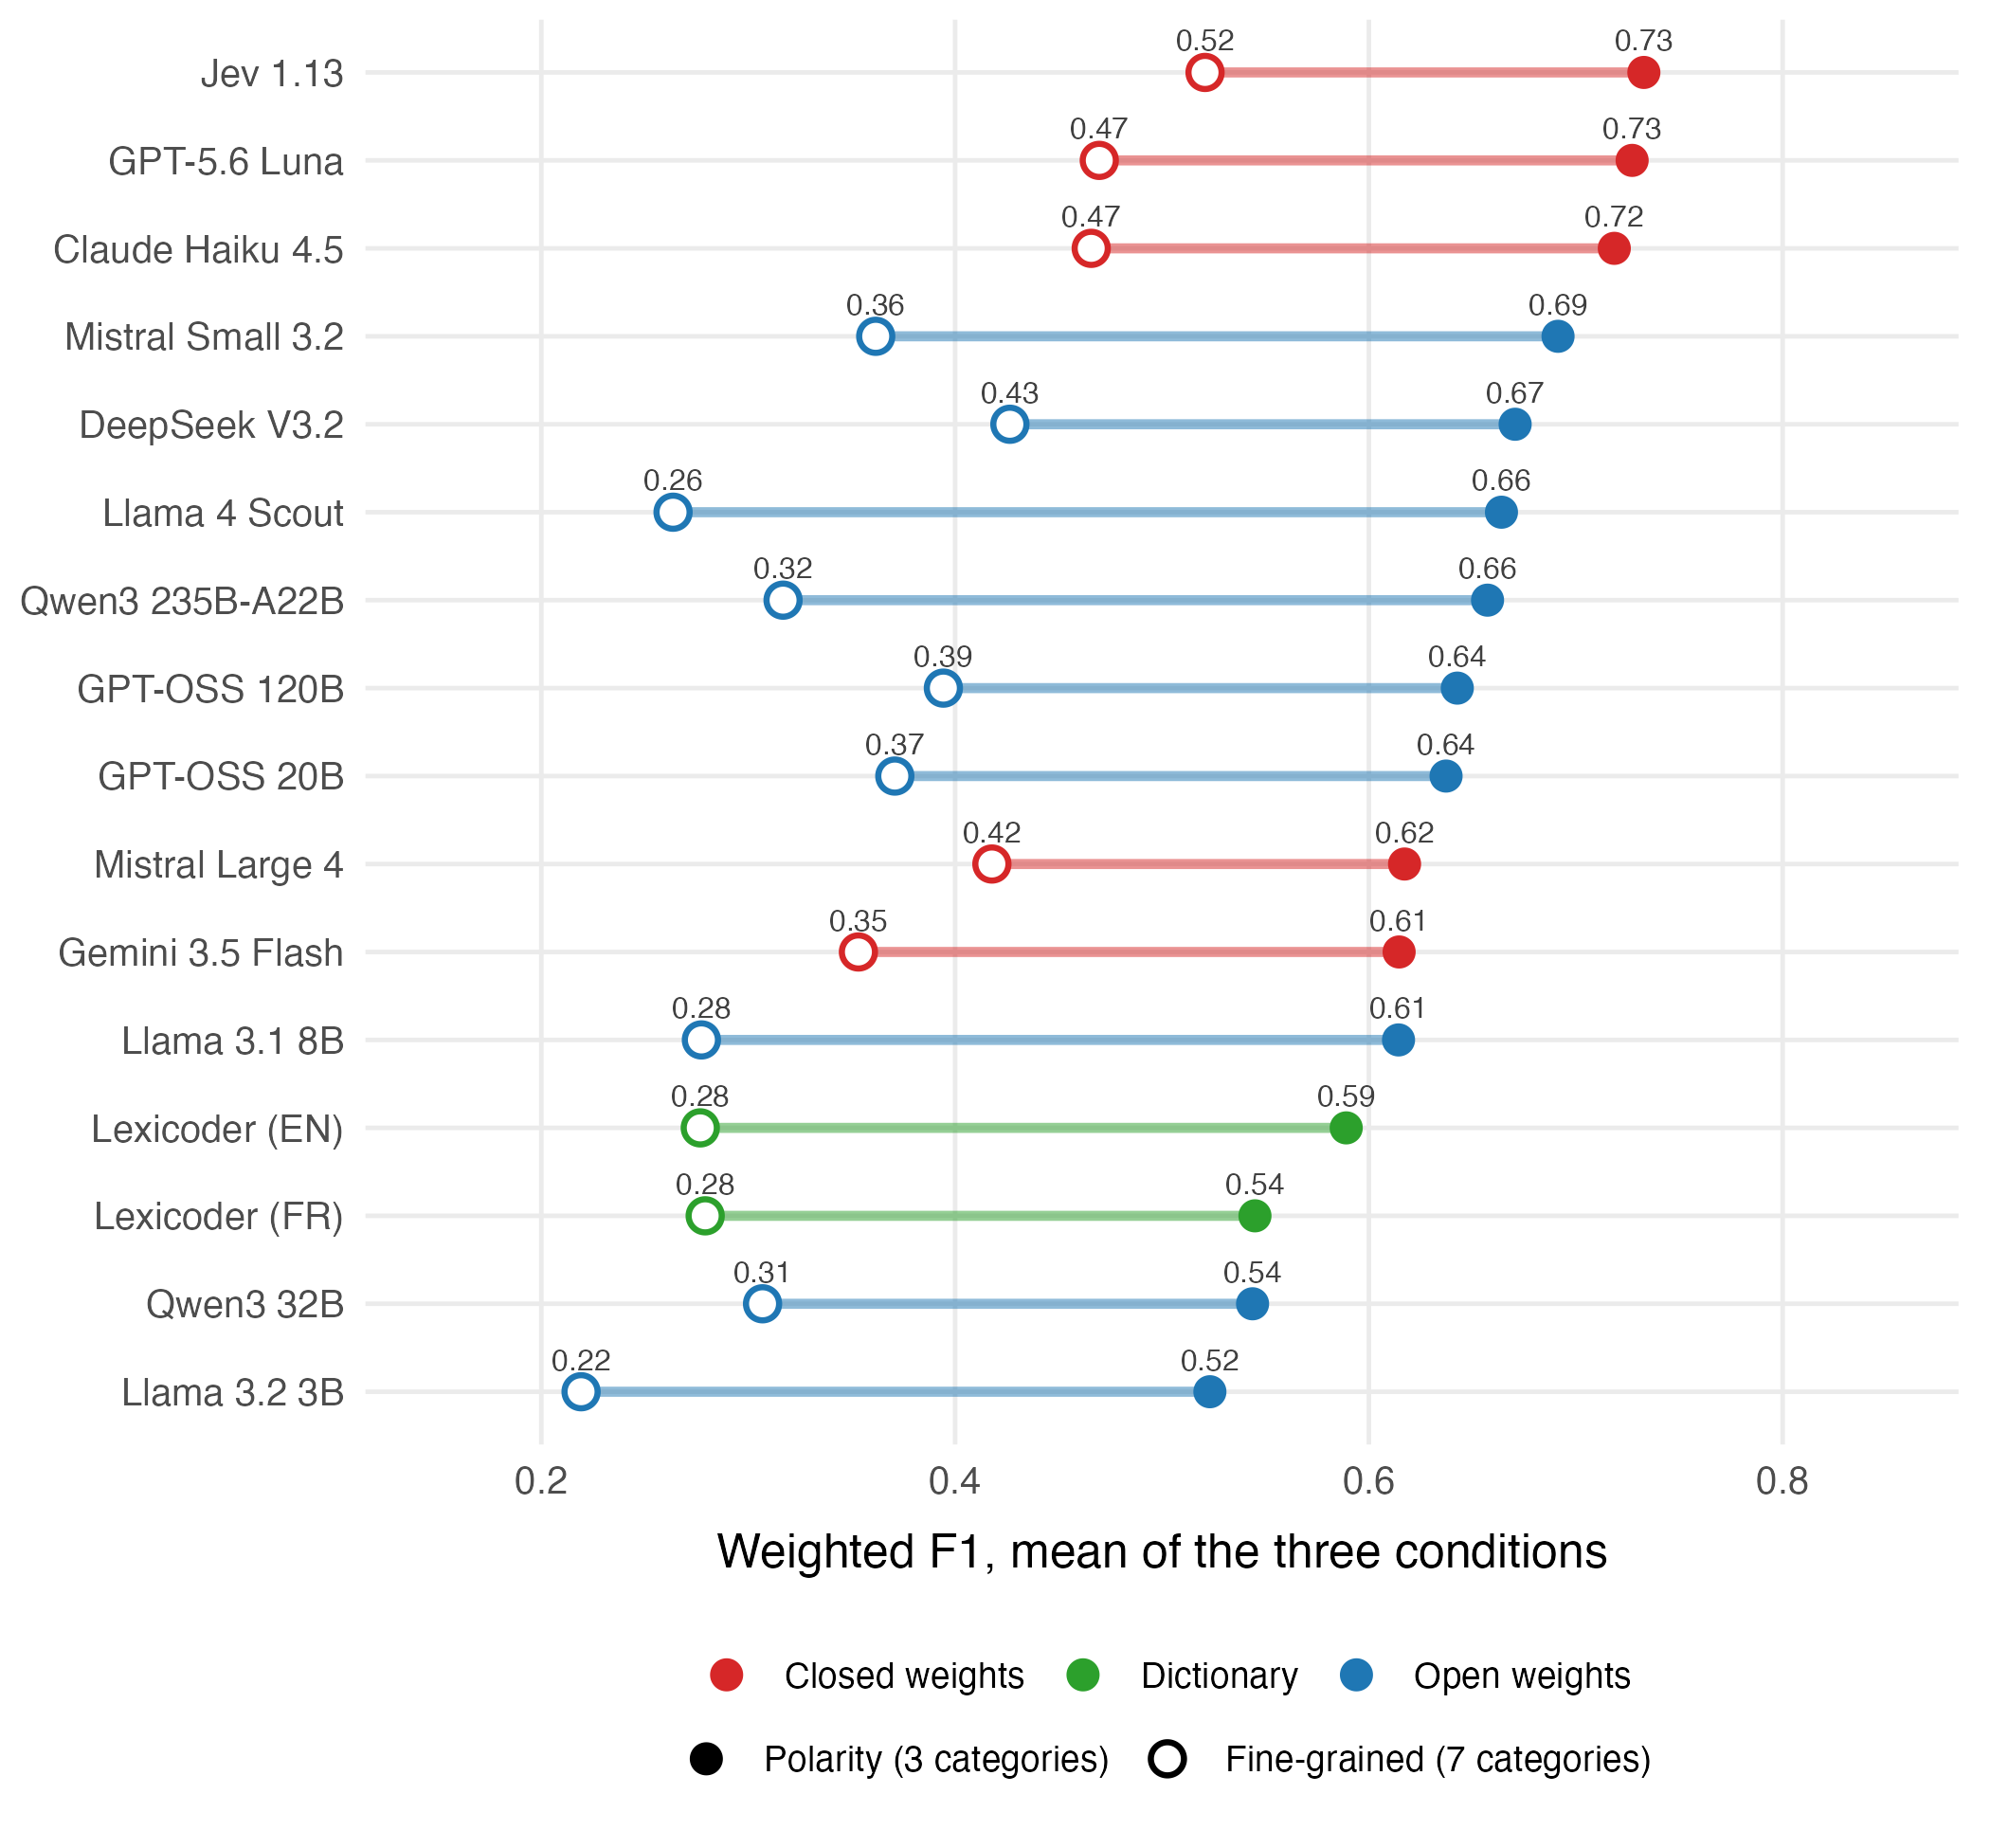
\includegraphics[keepaspectratio]{../../results/graphs/f1_dumbbell.png}}

\vspace{-12pt}
\noindent \emph{Note.} One~row per model, from the highest polarity F1
to the lowest, colored by model type. Filled circles are the weighted F1
on three categories, hollow circles on seven, each averaged over the
three conditions; the segment is the loss from grouping sentiment into
seven categories instead of three. Llama 3.2 1B is omitted.

\end{figure}

\begin{figure}[!htbp]

{\caption{{Agreement Between Scoring Methods on the Full Corpus, by
Article}{\label{fig-s-corpus}}}}

\pandocbounded{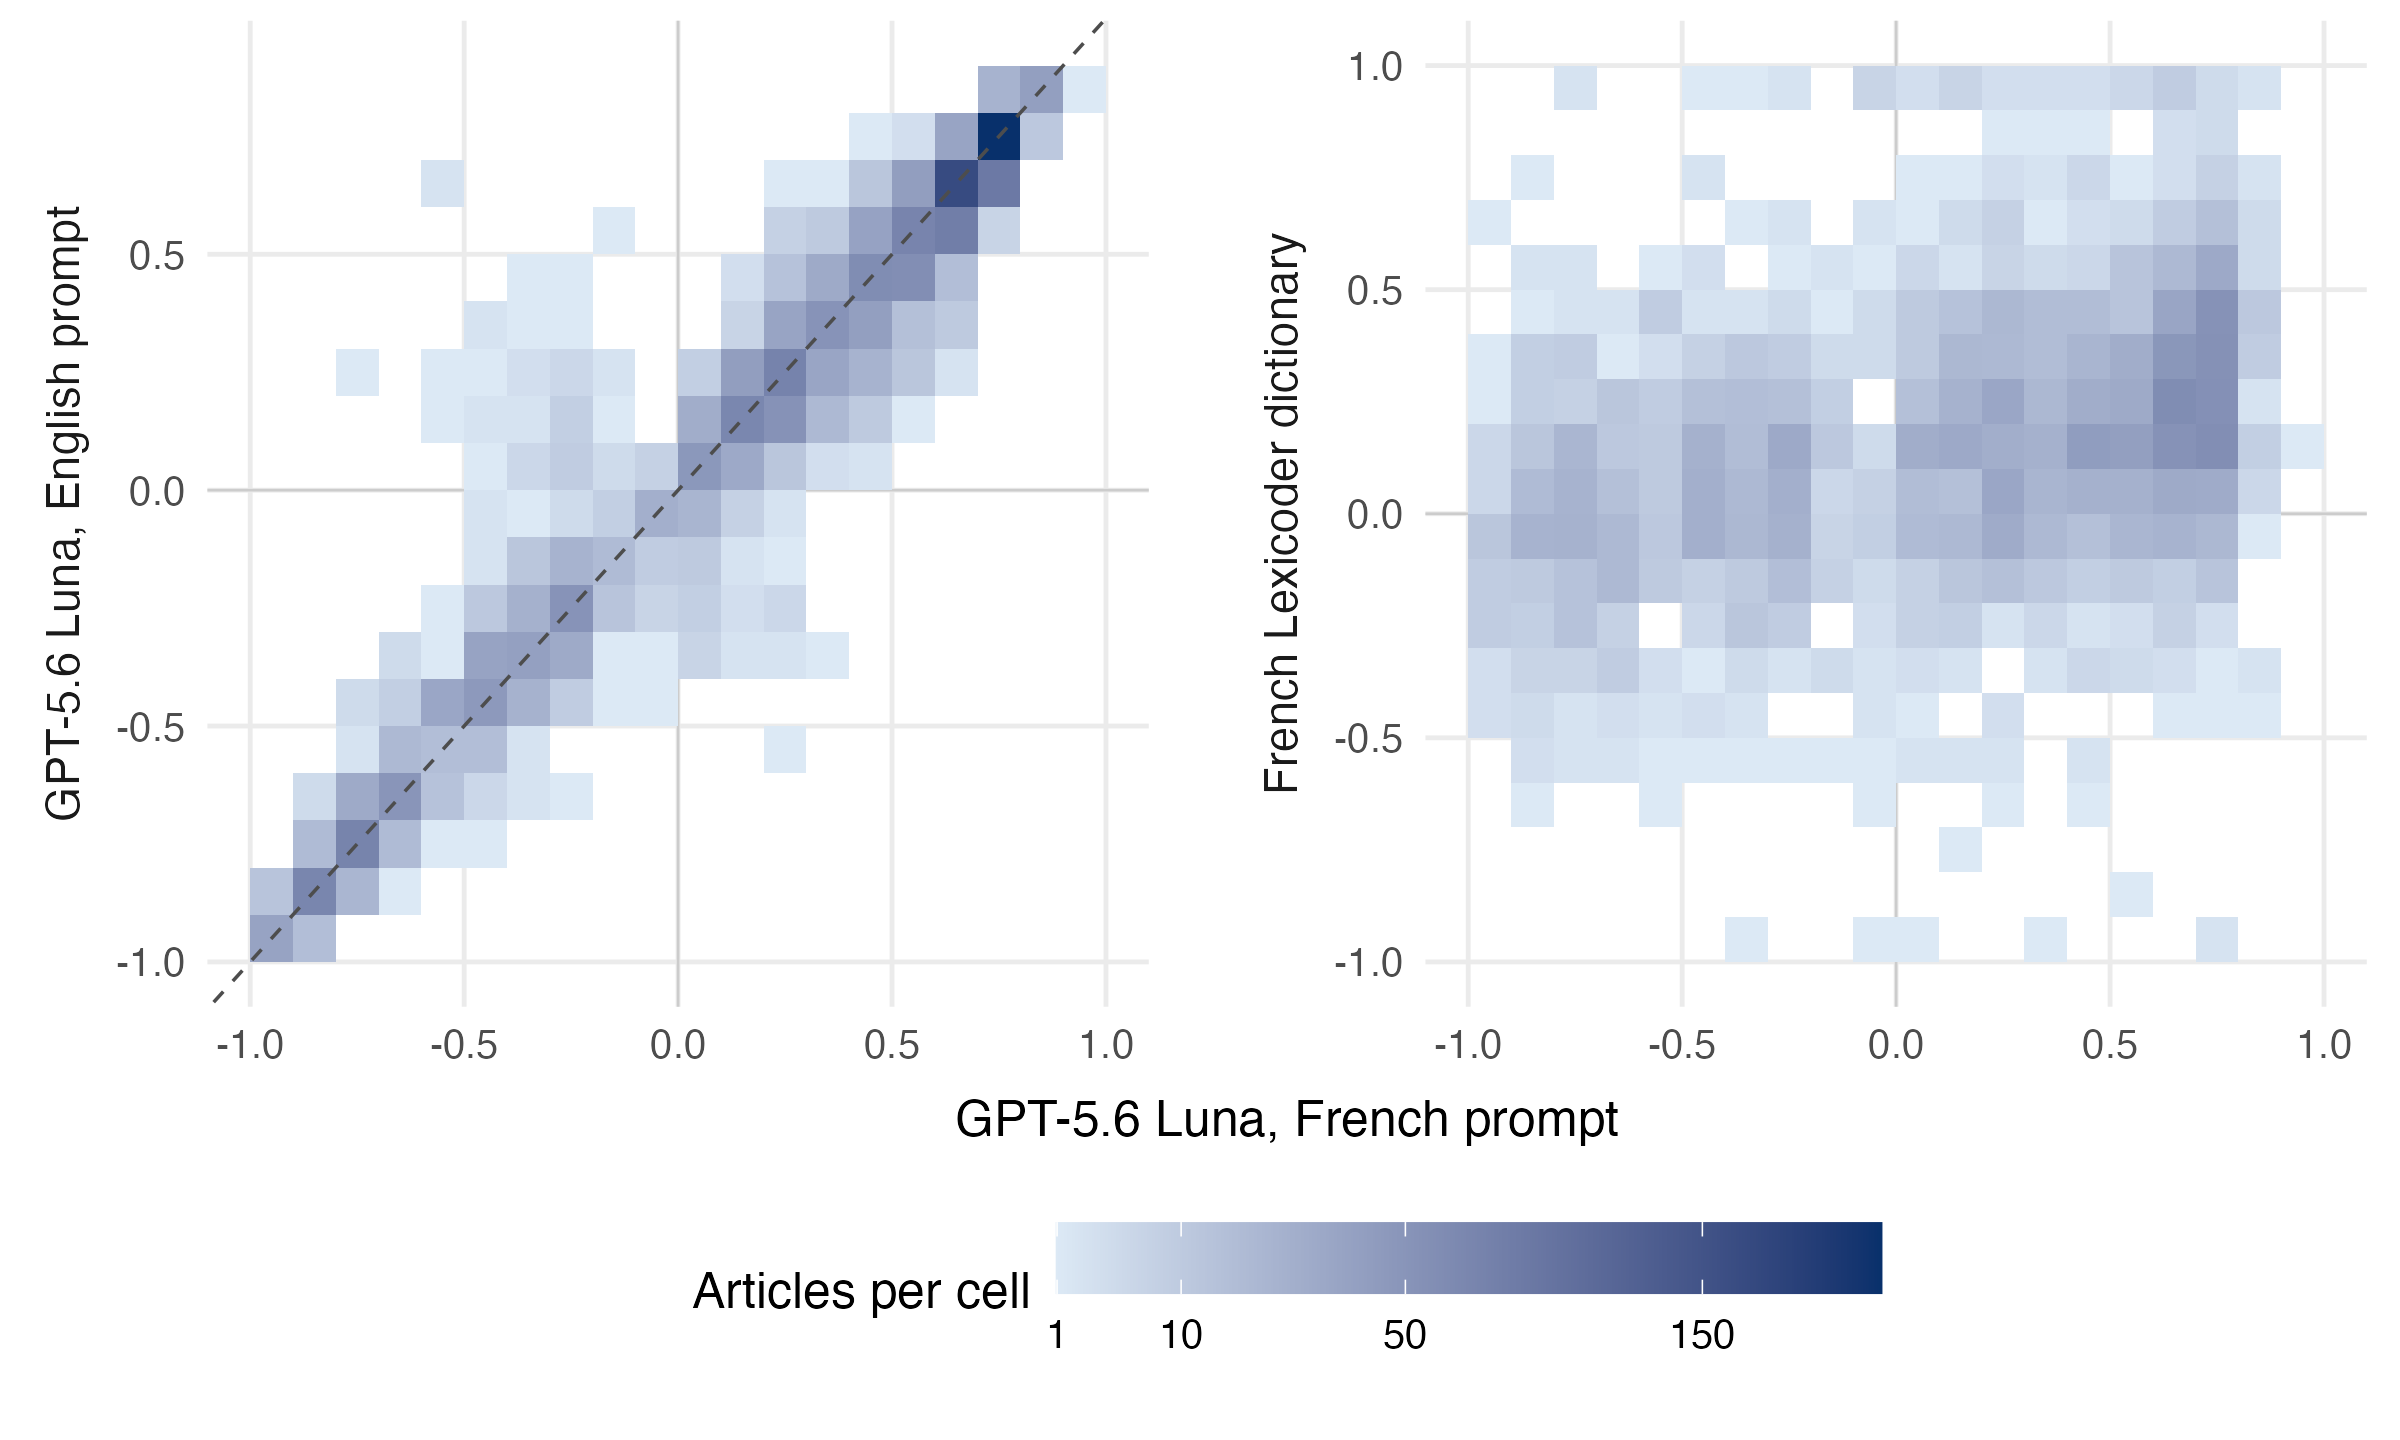
\includegraphics[keepaspectratio]{../../results/graphs/corpus_agreement.png}}

\vspace{-12pt}
\noindent \emph{Note.} Each~cell covers a 0.1 by 0.1 range of scores and
is shaded by the number of articles it contains (n = 2,671). The
horizontal axis is the GPT-5.6 Luna score under the French prompt. Left:
the same model's score under the English prompt, with the identity line
dashed (r = 0.97; the two prompts give the same sign on 94\% of
articles). Right: the French Lexicoder score on the original text (r =
0.36; the dictionary and the model give the same sign on 66\% of
articles and opposite signs on 28\%, the remainder being articles that
one of the two scores exactly zero). All scores run from −1 (very
negative) to 1 (very positive).

\end{figure}






\end{document}
